\documentclass[12pt]{beamer}

\mode<presentation>
{
  \usetheme{Madrid}     
  \usecolortheme{}
  \usefonttheme{default}  
  \setbeamertemplate{navigation symbols}{}
  \setbeamertemplate{caption}[numbered]
  \setbeamercolor{block title}{bg=orange!70}

} 

\usepackage[english]{babel}
\usepackage[utf8x]{inputenc}
\usepackage{amsmath,amsfonts,amsthm,graphicx}
\usepackage{bm,amsmath,bbm,amsfonts,nicefrac,latexsym,amsmath,amsfonts,amsbsy,amscd,amsxtra,amsgen,amsopn,bbm,amsthm,amssymb,textcomp,graphicx,float,verbatim,physics,hyperref,tabu, marvosym}
\usepackage[font=scriptsize]{caption}


\title[Rossby Waves]{Rossby Waves}
\author{Manu Sidhu, Sam Harrison, Philipp Breul, Edward Calver, Cathie Wells}
\institute{University of Reading and Imperial College London}


\begin{document}

\begin{frame}
  \titlepage
\end{frame}

\begin{frame}{Overview}
	
    \begin{itemize}
    	\item Introduce Rossby waves and the Shallow Water Equations (SWE). (Manu)
    	\item Potential Vorticity. (Philipp)
        \item Linearisation. (Sam)
        \item (Edward)
        \item Application of Rossby Waves. (Cathie)
    \end{itemize}
    
    \begin{figure}[H]
	    \centering
	    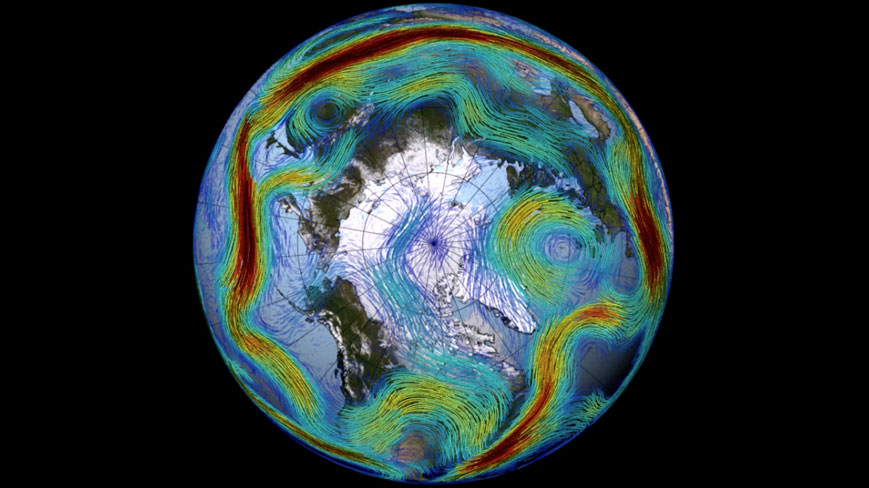
\includegraphics[width=0.5\linewidth]{Rossby_Wave.jpg}
    \end{figure}   
    
\end{frame}


\begin{frame}{Introduction - Rossby Waves}

\begin{itemize}
    \item Identified by Carl-Gustad Arvid Rossby.
    \item Large meanders in high altitude winds.
    \item Responsible for the weather at mid latitudes.
    \item Caused by the Earth's rotation.
    \item Two types of Rossby wave
\end{itemize}

\begin{table}[H]
	\begin{center}
		\begin{tabular}{ |c|c|} 
			\hline
			\textbf{Barotropic} & \textbf{Baroclinic} \\
			\hline 
			Free wave & Forced wave \\  
			Progress eastward and fast moving & Slow moving ($cm/s$) \\
			Free travelling & Quasi stationary \\
			No significant vertical changes & Vertical changes \\
			\hline
		\end{tabular}
	\end{center}
\end{table}

\begin{itemize}
    \item Caused by conservation of \textbf{potential vorticity}.
\end{itemize}

\end{frame}

\begin{frame}{How do we get to the Rossby Waves?}

\begin{itemize}
    \item Navier-Stokes \MVRightarrow  Shallow Water Equations (SWE) \MVRightarrow  Rossby Waves
\end{itemize}

\vspace{15pt}


The shallow water equation -
	\begin{equation}
    	\frac{\partial{\textbf{u}}}{\partial{t}} + \textbf{u}.\nabla\textbf{u} + f \textbf{z} \times \textbf{u} = -g \nabla h
    \end{equation}
    
The shallow water mass conservation - 

\begin{equation}
     	\frac{Dh}{Dt} + (h\nabla \textbf{u}) = 0.
    \end{equation}
    
\end{frame}


\begin{frame}{What are the Shallow Water Equations?}
	
    \begin{itemize}
    	\item A set of hyperbolic PDEs governing fluid flow in the oceans, coastal regions, rivers and channels.
        \item Consider the vertical length scale to be significantly smaller than the horizontal length scale.
        \item The SWE are derived from the Navier-Stokes equations.
		\item The Navier-Stokes equations are themselves derived from the equations for conservation of momentum (1) and the conservation of mass (2).
        \end{itemize}
        
    \vspace{-15pt}
        
 	\begin{equation}   
    	\rho(\frac{\partial{\textbf{u}}}{\partial{t}} + \textbf{u}.\nabla \textbf{u}) = -\nabla p  + \mu \nabla^2\textbf{u} + \rho \textbf{g},
    \end{equation}
 
 where $u=$ velocity, $p=$ pressure, $\rho=$ density and $\mu=$ viscosity.
 
 	\begin{equation}
     	\frac{\partial{\rho}}{\partial{t}} + (\nabla.\rho \textbf{u}) = 0.
    \end{equation}
 
\end{frame}


\begin{frame}{Deriving the Shallow Water Equations}

	\begin{itemize}
		\item Derive the Navier-Stokes equations from the conservation laws (1) and (2).
		\item Specify boundary conditions for the Navier-Stokes equations for a water column.
		\item Use the boundary conditions to depth integrate the Navier-Stokes equations.
    \end{itemize}
    
The Shallow Water Equation -
	\begin{equation}
    	\frac{\partial{\textbf{u}}}{\partial{t}} + \textbf{u}.\nabla\textbf{u} + f \textbf{z} \times \textbf{u} = -g \nabla h
    \end{equation}
    
	\begin{itemize}
		\item Linearise the system of equations to perform analysis on.
    \end{itemize}
    
\end{frame}



\end{document}